% SECTION 2.12: Audio FFT Pipeline. \input{} into the main report.
% PL hardware FFT (abandoned), host software FFT (adopted), comparison.
% Figures live in fft_image/ -- see capture notes in each caption.
\section{Audio FFT Pipeline}
\label{sec:audio_fft}

Two FFT implementations were explored to supply real-time spectral features to
the ray marcher: a Programmable Logic (PL) hardware FFT on the PYNQ-Z1 fabric,
and a host-side software FFT streaming pre-computed parameters over TCP. Both
deliver a feature vector every $\sim$23~ms to drive per-frame AXI-Lite register
updates; the software version was adopted (Sections~\ref{ssec:pl_fft},
\ref{ssec:host_fft}, \ref{ssec:fft_comparison}).

\subsection{PL FFT Implementation}
\label{ssec:pl_fft}

\subsubsection{Purpose and Design}
\label{sssec:fft_purpose}

The pipeline provides spectral features (bass/mid/treble energy fractions, RMS,
centroid, beat onset) fast enough for per-frame updates: at 1080p / $\sim$30~fps
a frame takes $\sim$33~ms, so a new vector was needed every 23--33~ms (one
1024-sample block at 44.1~kHz). The initial architecture placed the FFT in the
PL for potentially sub-millisecond latency (Figure~\ref{fig:pl_fft_block}): PS
audio samples went to a 1024-point FFT IP via AXI-DMA, magnitudes computed, then
DMA'd back for band-energy accumulation, freeing the ARM core for register
writes and the TCP server thread.

\begin{figure}[h]
  \centering
  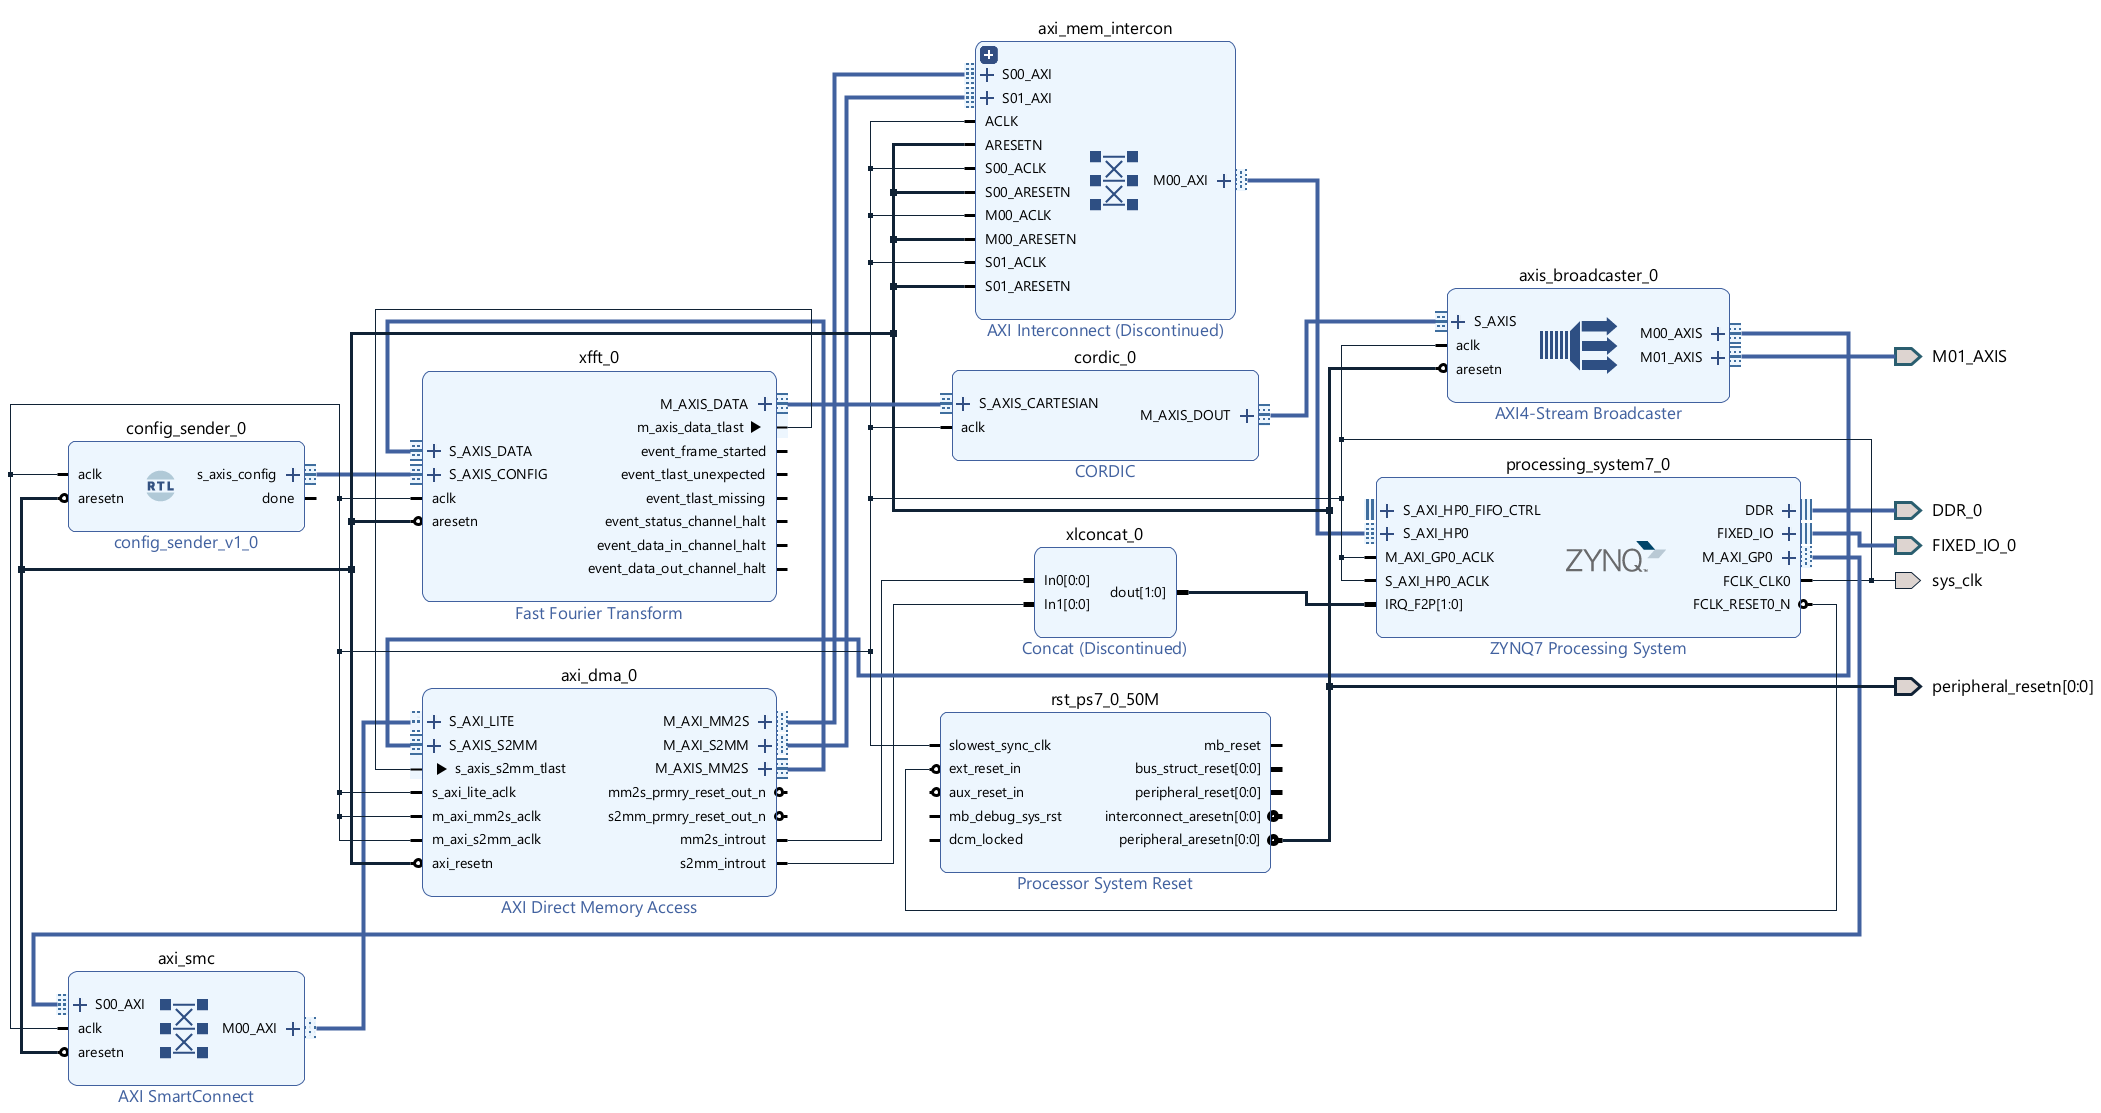
\includegraphics[width=0.8\linewidth]{imgs/fft_image/pl_fft_block.png}
  \caption{PL FFT pipeline block diagram (Vivado). Audio is staged through PS
  DDR and AXI-HP rather than an on-board input.}
  \label{fig:pl_fft_block}
\end{figure}

\subsubsection{FFT IP Configuration}
\label{sssec:fft_ip}

Xilinx's \textit{Fast Fourier Transform v9.1} IP was a fixed 1024-point
transform in \textit{Pipelined Streaming I/O} mode (one output per clock once
primed; at 100~MHz, $\sim$1100 cycles or $\sim$11~$\mu$s end-to-end). It used
complex input (imaginary tied to zero), 16-bit words, and \textit{Block Floating
Point} output (27-bit mantissa, matching FP27). Magnitudes
$|X[k]|=\sqrt{\text{Re}^2+\text{Im}^2}$ were computed in PS via a
\textit{CORDIC v6.0} IP; a 32-bit AXI-Stream pair carried data, with
\texttt{event\_*} signals monitored for overruns.

\begin{table}[h]
\centering
\caption{PL FFT IP resource utilisation (Vivado, xc7z020clg400-1).}
\label{tab:fft_resources}
\begin{tabular}{lrrr}
\toprule
\textbf{Resource} & \textbf{Used} & \textbf{Available} & \textbf{\%} \\
\midrule
LUT        & 3\,412 & 53\,200  & 6.4 \\
LUTRAM     & 248    & 17\,400  & 1.4 \\
FF         & 4\,106 & 106\,400 & 3.9 \\
BRAM (36k) & 5      & 140      & 3.6 \\
DSP48E1    & 22     & 220      & 10.0 \\
\bottomrule
\end{tabular}
\end{table}

These add to the ray marcher logic ($\sim$78\% LUT, 61\% FF, 85\% DSP), pushing
DSP utilisation to $\sim$95\% and causing hold-time violations on two paths that
needed manual placement constraints (Figure~\ref{fig:vivado_util}).

\begin{figure}[h]
  \centering
  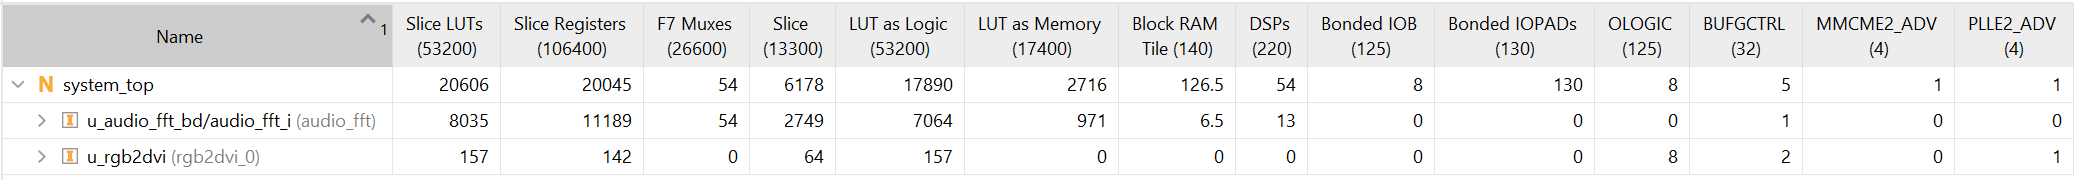
\includegraphics[width=0.8\linewidth]{imgs/fft_image/vivado_utilisation.png}
  \caption{Vivado post-implementation utilisation with the FFT IP added, DSP
  near saturation. (PL side --- capture in Vivado.)}
  \label{fig:vivado_util}
\end{figure}

\subsubsection{AXI-DMA and PS-Side Extraction}
\label{sssec:fft_dma}

Transfer used \textit{AXI DMA v7.1} in Simple mode over AXI-HP0: the PS callback
fills a 1024-sample ping-pong buffer; MM2S streams it to the FFT IP; S2MM writes
the 1025 output bins back; the PS computes magnitudes and accumulates bands.

Despite the $\sim$11~$\mu$s compute latency, measured DMA-start-to-result time
was \textbf{380--520~$\mu$s} per block, dominated by AXI latency, cache flushes
(\texttt{Xil\_DCacheInvalidateRange}), and polling. An interrupt-driven variant
(\textit{AXI INTC v4.1}) cut CPU cycles but added 100--200~$\mu$s of jitter, so
polling was retained.

\subsubsection{Frequency Band Definitions}
\label{sssec:fft_bands}

With $N=1024$ and $f_s=44100$~Hz the resolution is $\Delta f=f_s/N\approx43.1$~Hz.
Three perceptual bands (shared with the software FFT) were defined, bin~0 (DC)
excluded:

\begin{table}[h]
\centering
\caption{Frequency band definitions and FFT bin ranges.}
\label{tab:fft_bands}
\begin{tabular}{lccc}
\toprule
\textbf{Band} & \textbf{Range (Hz)} & \textbf{Bins} & \textbf{Count} \\
\midrule
Bass   & $43$--$215$   & $1$--$4$    & 4   \\
Mid    & $215$--$2000$ & $5$--$46$   & 42  \\
Treble & $2000$--$8000$& $47$--$185$ & 139 \\
\bottomrule
\end{tabular}
\end{table}

Boundaries used $k=\mathrm{round}(fN/f_s)$ (clamped to $\geq1$), with energies
normalised by total power so PL and software feature vectors match.

\subsection{Host-Side Software FFT}
\label{ssec:host_fft}

The host PC analyses live audio (mic or loopback) every 1024-sample block,
extracts seven features via FFT, maps them to SDF scene parameters, and streams
the result to the PYNQ-Z1 over TCP, whose ARM core writes the values into the
ray marcher's AXI-Lite registers (Figure~\ref{fig:sw_pipeline}).

\begin{figure}[h]
  \centering
  \begin{tikzpicture}[font=\footnotesize, node distance=4mm and 6mm, >={Stealth[length=2mm]},
      box/.style={draw, rounded corners=2pt, align=center, inner sep=3pt, minimum height=8mm, text width=20mm},
      host/.style={box, fill=blue!6}, net/.style={box, fill=orange!12, text width=16mm}, board/.style={box, fill=green!8}]
    \node[host] (cap) {Audio capture\\\texttt{sounddevice}\\1024 @ 44.1\,kHz};
    \node[host, right=of cap] (cond) {Downmix mono\\int16 fix};
    \node[host, right=of cond] (fft) {\texttt{rfft}\\$|X[k]|$};
    \node[host, right=of fft] (feat) {7 features\\bands, RMS,\\cent, beat, ZCR};
    \node[host, below=8mm of feat] (map) {Scene map\\\texttt{cell\_sz},\texttt{b\_fp},\\\texttt{e\_fp}, cam pos};
    \node[net, left=of map] (pack) {Pack 11$\times$\\\texttt{float32}\\(44\,B)};
    \node[net, left=of pack] (tcp) {TCP\\port 9998};
    \node[board, left=of tcp] (recv) {\texttt{board.py}\\\texttt{recv(44)}\\\texttt{MSG\_WAITALL}};
    \node[board, below=8mm of cap] (conv) {\texttt{fp32\_to\_fp27}};
    \node[board, right=of conv] (mmio) {MMIO write\\regs 9--22\\(AXI-Lite)};
    \draw[->] (cap) -- (cond); \draw[->] (cond) -- (fft); \draw[->] (fft) -- (feat);
    \draw[->] (feat) -- (map); \draw[->] (map) -- (pack); \draw[->] (pack) -- (tcp);
    \draw[->] (tcp) -- (recv); \draw[->] (recv) |- (conv); \draw[->] (conv) -- (mmio);
    \node[anchor=south west, font=\scriptsize\itshape, blue!55!black] at (cap.north west) {Host PC (PS-side software)};
    \node[anchor=north west, font=\scriptsize\itshape, green!45!black] at (conv.south west) {PYNQ-Z1 board};
  \end{tikzpicture}
  \caption{Host-side software pipeline (top, blue) feeding the board (bottom,
  green): capture $\to$ FFT $\to$ features $\to$ scene map $\to$ pack $\to$ TCP,
  then FP27 conversion and AXI-Lite register writes.}
  \label{fig:sw_pipeline}
\end{figure}

\subsubsection{Audio Capture}
\label{ssec:capture}

\texttt{audio\_sender.py} uses \texttt{sounddevice} (a PortAudio binding) in
callback mode. PortAudio exposes each endpoint once per host API, so the choice
affects latency and available virtual devices:

\begin{table}[h]
\centering
\caption{Windows audio host APIs via PortAudio.}
\label{tab:apis}
\begin{tabular}{lllp{4.4cm}}
\toprule
\textbf{API} & \textbf{Latency} & \textbf{Stereo Mix} & \textbf{Notes} \\
\midrule
MME          & 30--100~ms & Yes & Legacy; most compatible fallback \\
DirectSound  & $\sim$20~ms & Yes & Emulated over WASAPI; no benefit \\
WASAPI shared& $\sim$20~ms & Yes & Modern; recommended \\
WDM-KS       & $<$5~ms    & No  & Kernel-level; no Stereo Mix; may scale floats to int16 \\
\bottomrule
\end{tabular}
\end{table}

We use \textbf{WASAPI shared mode}: $\sim$20~ms latency (ample for $\sim$23~ms
blocks), normalised float samples, and Stereo Mix as a loopback source. WDM-KS
drivers sometimes deliver \texttt{float32} at int16 scale, corrected by
$x[n] \leftarrow x[n]/32768$ if $\max_n|x[n]|>2$. \textit{Stereo Mix}, a Realtek
virtual endpoint capturing the final mixed playback, is enabled via
\texttt{mmsys.cpl} $\to$ Recording $\to$ Show Disabled Devices, then selected
with \texttt{--device "Stereo Mix"}. Each callback delivers $N=1024$ samples at
$f_s$ ($\sim$44100~Hz); stereo is downmixed to mono ($x[n]=\frac1C\sum_c x_c[n]$)
and the int16-scale anomaly corrected --- the only pre-processing before the FFT.

\subsubsection{FFT and Spectral Feature Extraction}
\label{ssec:fft}

A real-valued FFT is computed per block, with
$X[k]=|\sum_{n=0}^{N-1} x[n]\,e^{-j2\pi kn/N}|$ for $k=0,\dots,\tfrac{N}{2}$.
Band energies are normalised by total power so they are volume-independent:
\begin{equation}
E_{\mathrm{total}}=\textstyle\sum_k X[k],\quad
B_{\mathrm{band}}=\frac{\sum_{k\in\text{band}}X[k]}{E_{\mathrm{total}}}
\end{equation}
for bass ($43$--$215$~Hz), mid ($215$--$2000$~Hz), treble ($2000$--$8000$~Hz). A
\emph{silence gate} zeroes ratio features when $E_{\mathrm{total}}<\theta_s=0.3$,
and energies are smoothed by a first-order IIR filter
$\hat{B}[t]=\alpha B[t]+(1-\alpha)\hat{B}[t-1]$, $\alpha=0.3$ ($\tau\approx70$~ms).

Four further features are extracted: \textbf{RMS amplitude}
$\min(\sqrt{\frac1N\sum_n x[n]^2},1)$ (loudness $\to$ orbit radius);
\textbf{spectral centroid}
$C_{\mathrm{norm}}=\min(\frac{\sum_k f_k X[k]}{\sum_k X[k]+\epsilon}/8000,1)$,
$f_k=kf_s/N$ (brightness $\to$ camera height); \textbf{beat onset} when
$E[t]>1.5\,\overline{E}_{20}$; and \textbf{zero-crossing rate} (a spare
noisiness parameter).

\subsubsection{Scene Parameter Mapping}
\label{ssec:mapping}

For the box-frame lattice scene (Section~\ref{sec:sdf_scene}):
\begin{align}
\texttt{cell\_sz} &= 10.0 + \hat{B}_{\mathrm{bass}}\cdot4.0, &
\texttt{b\_fp}    &= 4.5  + \hat{B}_{\mathrm{mid}}\cdot1.5, &
\texttt{e\_fp}    &= 0.15 + \hat{B}_{\mathrm{treble}}\cdot0.1.
\end{align}
The camera orbits in XZ at $\Delta\phi=(0.5\hat{B}_{\mathrm{bass}}+0.05)N/f_s$,
with $R=8.0-3.0\,\mathrm{RMS}$ and $p_y=0.15+C_{\mathrm{norm}}$; the 11 packed
values are dispatched each callback.

\subsubsection{TCP Streaming Protocol}
\label{ssec:protocol}

The host (client) connects to the board (server) on TCP port 9998. The protocol
is minimal: one fixed 44-byte frame per callback --- eleven \texttt{float32} LE
values (camera $p_x,p_y,p_z$; \texttt{cell\_sz}; \texttt{b\_fp}; \texttt{e\_fp};
RMS; centroid; beat; ZCR; one reserved) --- with no header, sequence, or ack,
packed via \texttt{struct.pack("11f", *values)}. The receiver reads exactly 44
bytes with \texttt{MSG\_WAITALL}; a short read is a clean disconnect, after which
the server re-enters \texttt{accept()}. Frames are self-contained, so
reconnection needs no state reset.

\subsubsection{Board-Side Connection and Register Writes}
\label{ssec:board}

\texttt{board.py} runs on the PYNQ-Z1 under Python~3. Its server thread loops:
\begin{verbatim}
conn, addr = server.accept()
while True:
    data = conn.recv(44, MSG_WAITALL)
    if len(data) != 44: break          # disconnect
    for i, v in enumerate(struct.unpack("11f", data)):
        mmio.write((9 + i) * 4, fp32_to_fp27(v))
\end{verbatim}

Each value is converted to the ray marcher's custom 27-bit float (1 sign, 8
exponent, 18 mantissa) before the MMIO write, truncating the mantissa from 23 to
18 bits with round-to-nearest
($\texttt{frac}_{18}=\lfloor(\texttt{frac}_{23}+2^4)/2^5\rfloor$); subnormals
flush to zero, inf/NaN pass through. The camera origin occupies registers 9--11
and the eight \texttt{sdf\_params} registers 15--22, leaving the lookat matrix
(0--8) to the IMU thread. \texttt{board.py --no-hw} substitutes a
\texttt{DummyMMIO} that prints register snapshots, validating the pipeline
without hardware. The dominant latency is the audio block
($1024/44100\approx23$~ms); TCP over USB RNDIS adds $\sim$1~ms and MMIO a few
$\mu$s, giving \textbf{$\sim$25--30~ms} total --- well below the
$\lesssim$100~ms perceptual threshold.

\subsection{Comparison and Design Decision}
\label{ssec:fft_comparison}

\begin{table}[h]
\centering
\caption{PL FFT (PYNQ-Z1 fabric) vs.\ software FFT (host PC, NumPy/FFTW).}
\label{tab:fft_comparison}
\begin{tabular}{lp{4.6cm}p{4.6cm}}
\toprule
\textbf{Criterion} & \textbf{PL FFT} & \textbf{Software FFT (adopted)} \\
\midrule
Compute latency & $\sim$11~$\mu$s (kernel only) & $<$0.5~ms (NumPy \texttt{rfft}) \\[3pt]
End-to-end & 380--520~$\mu$s (AXI-DMA + cache flush) & $\sim$24--25~ms (block + TCP) \\[3pt]
PL resource & +6.4\% LUT, +10\% DSP $\to$ $\sim$95\% DSP, hold violations & Zero PL usage \\[3pt]
Complexity & DMA, cache coherency, IRQ/poll, CORDIC, ping-pong & Single \texttt{rfft()} call \\[3pt]
Audio source & Needs I\textsuperscript{2}S/PDM hardware (not on-board) & Host audio subsystem; Stereo Mix loopback \\[3pt]
Features & 3 bands + RMS & 7 features, easily extensible \\[3pt]
Portability & Coupled to Zynq IP; re-synthesis per change & Pure Python; edit constants \\[3pt]
Validation & Hardware-in-the-loop required & \texttt{--no-hw} stub on any machine \\
\bottomrule
\end{tabular}
\end{table}

Across every criterion except raw kernel latency the software version equals or
beats the PL design (that edge erased by AXI-DMA overhead), abandoned for three
reasons:

\begin{enumerate}
  \item \textbf{Resource conflict.} The FFT IP raised DSP48 utilisation to
  $\sim$95\%, unplaceable without hold-time violations; the fix left $<$2\% slack.
  \item \textbf{Illusory latency.} The $\sim$11~$\mu$s kernel was swamped by
  370--510~$\mu$s of AXI-DMA overhead; against a 23~ms block, 0.5~ms is moot.
  \item \textbf{No audio input path.} The PYNQ-Z1 has no on-board mic or line in;
  feeding the PL FFT needs an I\textsuperscript{2}S daughter-board or PCM staged
  from the host anyway --- at which point the host can do the FFT for free.
\end{enumerate}

Moving the FFT to the host fixed all three: PL utilisation returned to safe
levels, the seven features extract in $<$0.5~ms, and latency stays $\sim$25--30~ms.
